\documentclass{article}
\usepackage[utf8]{inputenc}
\usepackage{hyperref}
\usepackage{xcolor}
\usepackage{graphicx}
\graphicspath{ {./images/} }

\hypersetup{
    colorlinks,
    citecolor=black,
    filecolor=black,
    linkcolor=black,
    urlcolor=blue
}


\definecolor{light-gray}{gray}{0.95}
\newcommand{\code}[1]{\colorbox{light-gray}{\texttt{#1}}}
 
\title{RSA Encryption Final Project}
\author{Ariel Young, Nashir Janmohamed}
\date{June 14, 2020}
  
\renewcommand*\contentsname{Summary}

\begin{document}

\maketitle
\tableofcontents

\section{Introduction}
The goal of this project was to re-implement the RSA hashing algorithm in Rust, separately from the existing crate. Initially, our goal was to have a cryptographically secure implementation of RSA. While at first we thought that we had achieved this goal, upon further review, there turned out to be several notable issues with our implementation, mainly relating to random number generation.

\section{Theory}
\subsection{RSA Algorithm}
Given two very large (in our case, 512-bit, \char`\~ 150 digit) prime numbers $p$ and $q$, the product $n = pq$ cannot be factored in any reasonable amount of time using modern computing hardware (due to the lack of an efficient factoring algorithm). This is the basis for the RSA cryptographic system. \textit{TODO: This paragraph needs work, expansion}

In addition to $n$, the two other components required by RSA are the encryption exponent, $e$, and the decryption exponent, $d$. We should choose $e$ such that $e$ is coprime to the product $(p - 1)(q - 1)$. An accepted practice is to choose a constant prime value for $e$, rather than computing a random coprime value. In our implementation, we have set $e$ to be the constant $2^{16} + 1 = 65,537$. This choice of $e$ is generally regarded as more secure than smaller primes, and also allows for more efficient decryption \cite{rsa_attacks}. The public key is formed by the pair $(n,\, e)$.

After having chosen $p$, $q$, and $e$, we can compute our decryption exponent $d$, such that: \[ d*e \equiv 1 \;(\textbf{mod}\,(p - 1)(q - 1)) \] In our implementation, we are computing the solution for $d$ by using the Extended Euclidian Algorithm to solve for the coefficients of Bézout's identity, which is both more efficient and far more scalable than other approaches. This increased efficiency was necessary because of the size of the primes our implementation uses. The private key is formed by the pair $(n,\, d)$.

From here, the rest of the algorithm is relatively simple. After packing the characters from a message into integers (we used 32 bit integers, each of which holds 4 ASCII characters), the cipher $c_i$ for each packed block $m_i$ can be computed using the formula:
\[ c_i = m_i^e\, \textbf{mod} \, n \]
Although our implementation does not have this feature (we store ciphers as arrays of unsigned 8-bit integers in JSON files for transport), the ciphers can be reassembled into one string. Many implementations also perform some form of symmetric encryption on this string before outputting it.

In order to decrypt, we can find the packed value $m_i$ from each cipher block $c_i$ using the formula:
	\[ m_i = c_i^d \,\textbf{mod}\, n \]
At this point, the original text of the message can be unpacked and fully recovered.

\subsubsection{Random Number Generation}
To implement random number generation, we used the Linear Congruential Method. This is a recursive sequence of pseudo-random numbers, defined by the relation:
\[ x_n = (ax_{n - 1} + c) \textbf{ mod } m \]
In this relation, $a$ is a multiplicative constant, $c$ is an additive constant, and $m$ is the modulus (also a constant). For these values, we have chosen to mirror those used by the implementation of the Linear Congruential Method in Gnu's \code{glibc}. Our seed $x_0$ is the current Unix time, in microseconds. In order to normalize the output of our random number generator, we divide by the modulus before returning the result of each iteration, which returns an output in the range $[0,\, 1)$.

An important note is that our random number generator is most definitely not secure. While it passes the Chi-squared test, we still have a direct linear dependence on the initial seed, which secure implementations (particularly glibc) usually avoid with an additional recursive term \cite{lcm}. Our generator would most likely fail the Spectral test \cite{spectral}.

\subsubsection{Generating Large Primes}
Initially, we had intended to use prime number sieves and random selection to generate our primes $p$ and $q$. Various approaches were investigated, including using the \textit{Sieve of Eratosthenes} \cite{sieveeratosthenes}, and then the \textit{Sieve of Atkin} \cite{sieveatkin} when we realized that Eratosthenes was not sufficiently efficient. However, this approach has two main flaws. The first of these is that prime number sieves generate \textit{all} prime numbers under a certain boundary, and random selection from these sets could yield two values of drastically different sizes. Optimally, $p$ and $q$ should differ by (at most) a few orders of magnitude. The second (and more notable) flaw was that we only needed two primes, not all primes below some limit. Moreover, these primes must be extremely large, of a size where sieves become entirely impractical.

Thus, we eventually settled on implementing the Miller-Rabin primality test. The Miller-Rabin primality test is an extension of Fermat's primality test, which in turn makes use of Fermat's little theorem. The Miller-Rabin test, although it is probabilistic rather than deterministic, corrects for the case in which Fermat's little theorem fails (for numbers that aren't coprime) \cite{millerrabin}, and returns (within some degree of certainty) whether or not a particular number is prime. For large numbers, with a resonable number of iterations, the likelihood that the Miller-Rabin primality test fails is approximately equivalent to the likelihood that some random bit flip due to cosmic rays introduces an error to relevant memory while the calculations are performed (see \textbf{\hyperref[sec:rays]{notes}}).


\section{Analysis}
\subsection{Chi-Squared Test}
\label{chi}
After computing the Chi-squared value for our random number generator, over the course of several thousand iterations performed on disparate (i.e., differently seeded) generators, the resultant $p$-value is uniformly very close to zero, which would seem to imply that our distribution is truly random. However, the Chi-squared test is not definitive for random number generators; many generators which pass Chi-squared do not pass the Spectral test.

\subsection{Bitmap}
Another way to assess the performance of a random number generator is by inspection. A bitmap visualization of the output of the random number generator (which produces values in the range [0,1)) was created with each pixel assigned a value of 0 or 1 - 0 if the generated value is less than 0.5, and 1 otherwise. Though a seemingly imprecise and qualitative test in comparison to the more quantitative Chi-squared test [ref \nameref{chi}] or the Spectral test \cite{spectral}, according to Matson \cite{matson}, the ability of the human brain to recognize patterns is the fundamental basis of human intelligence. Visualizing successive results of the RNG gives an alternative means of assessing the ``randomness''.

\subsection{Runtime Analysis}
Our implementation of RSA is slow. Theoretically, it should not be that slow. The big-O of our algorithm overall is more or less to the tune of $O(n^2)$. However, in practice, it is slower than a geriatric slug. This is largely due to the shot-in-the-dark approach we're taking to prime generation (we could also filter obvious composites using a faster method before applying Miller-Rabin), and all of the memory copies forced upon us by Rust's concept of ownership. \textit{Remove this section? Not sure how to formalize}


\section{Usage}
\subsection{CLI}
In order to facilitate "playing" with our implementation of RSA, we created a text-based command line interface (``CLI") that is vaguely reminiscent of that of GPG. It includes the capability to generate a new key, encrypt a message using that key, and then write both the public and private keys, and also the message cipher, to disk. Additionally, it can read back from disk the message cipher and private key, and reproducably decrypt the cipher. I will demonstrate this process below.

A prebuilt macOS binary of our project can be found \href{https://github.com/DarthGeek01/rust-rsa-vis/releases/tag/v0.0}{at this link}. It is the file called \code{rsa\_vis}. One should be able to simply download it, and then double click to open the CLI.
\\\\\\\\\\
Upon opening the file, we should be  greeted with something that looks more-or-less like this: \\
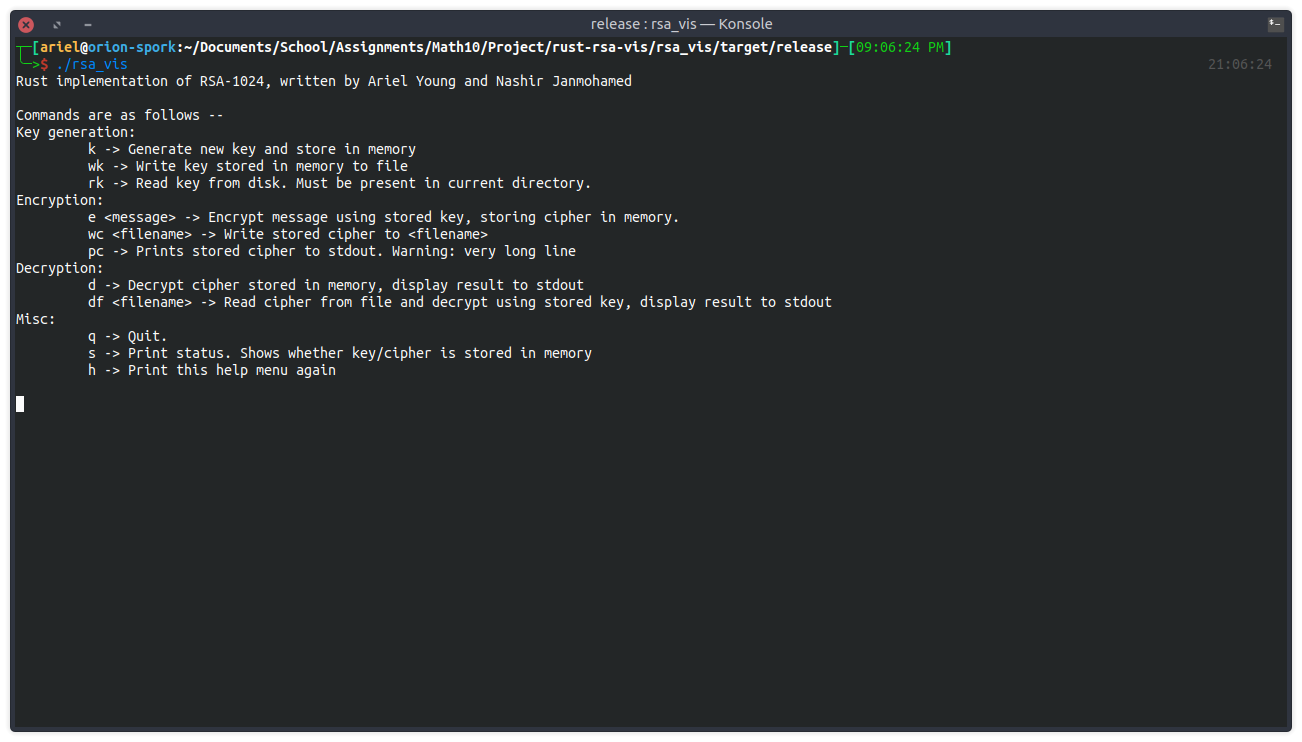
\includegraphics[width=\textwidth]{one}

At this point, we should enter the command \code{k}, in order to generate a new key. After doing so, we can the proceed to encrypt a message using the command \code{e <message>}. The message can include any ASCII characters. For the sake of the example, we'll encrypt the message ``Hello, world!". At this point, the result of the encryption (in bytes stored as unsigned 32-bit integers) will be printed to the console: \\
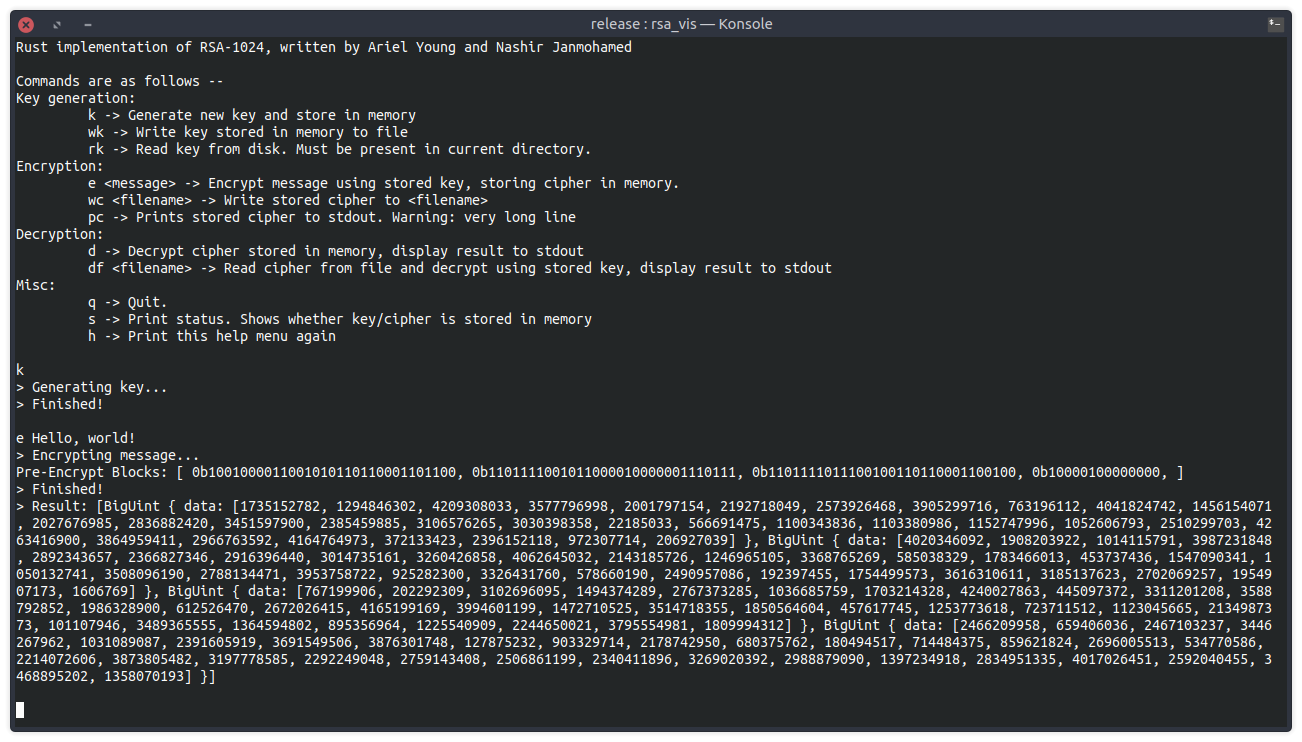
\includegraphics[width=\textwidth]{two}

At this point, we can enter the commands \code{wk}, and then \code{wc cipher.txt}, to write the key and cipher to disk, respectively. Note that one limitation of the current implementation is that the keys will be written to preset file names in the current directory. After writing both key and cipher to disk, we can exit the program using \code{q}, and then relaunch it.

After relaunching the program, we should be greeted with the same dialog that greeted us the first time that we launched the program. We can then enter \code{rk} to read the public and private keys back from disk. At this point, we should be able to enter the command \code{df cipher.txt} to read the cipher from disk, and then decrypt it. If all goes well, the output should look something like this:
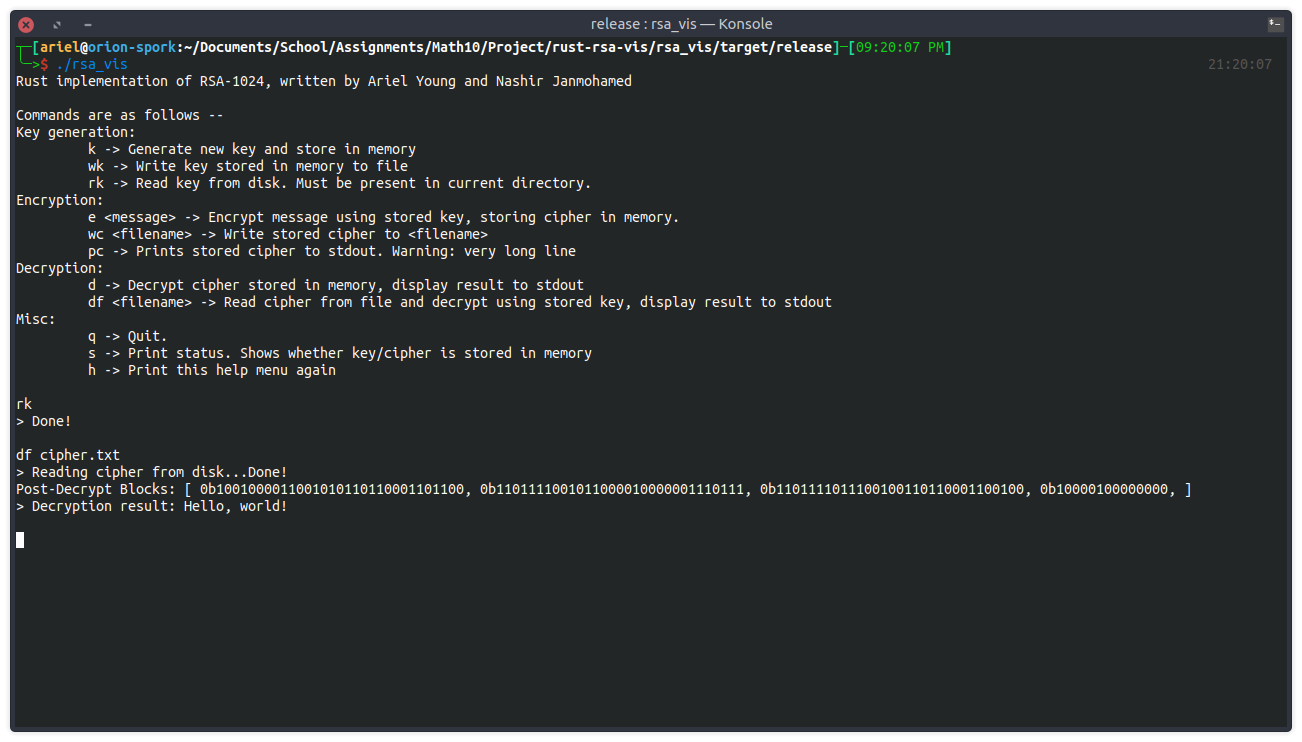
\includegraphics[width=\textwidth]{three}

For posterity, I shall also demonstrate that, if a new key is generated, the old cipher can no longer be decrypted. After decrypting the file, we should enter the command \code{k} again, to generate a new key, and then enter the command \code{df cipher.txt} in order to attempt to decrypt the file again. The output should consist of several error messages and an empty result: \\
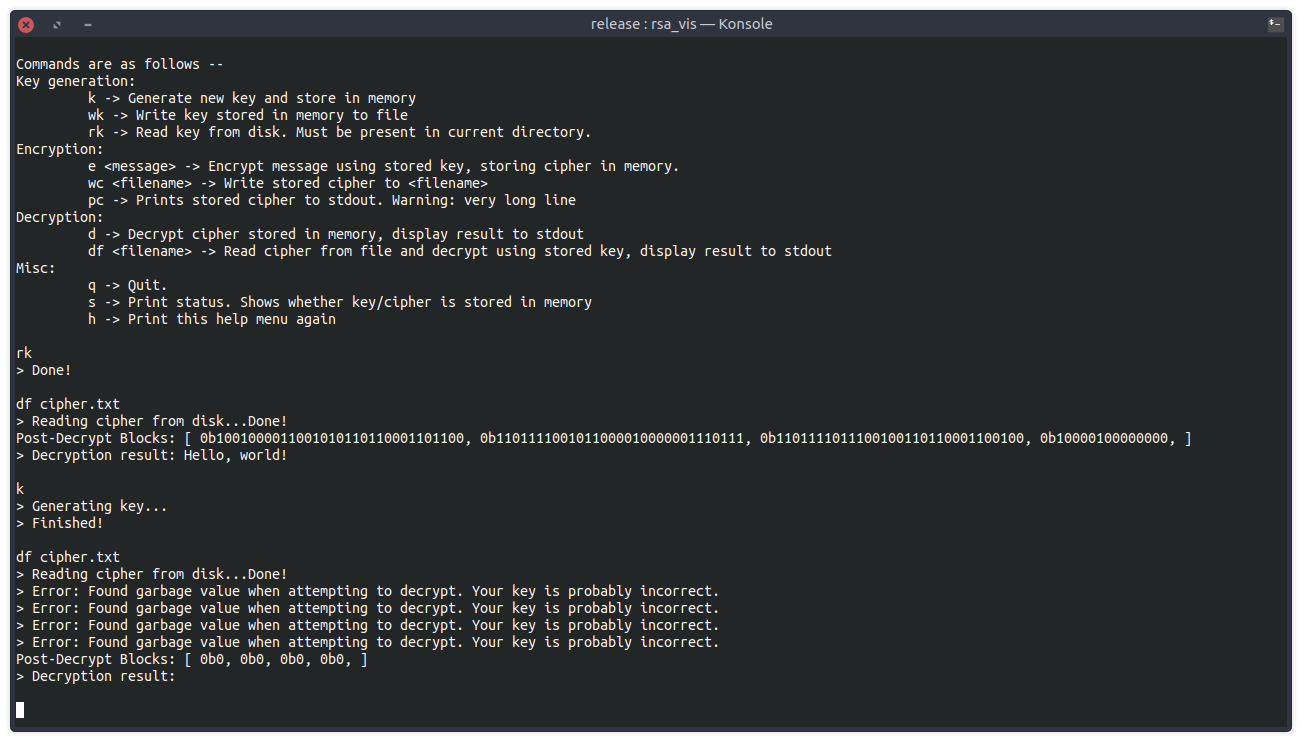
\includegraphics[width=\textwidth]{four}

Thus concludes the usage demonstration of our CLI. While there are other available commands, they are all relatively self-explanatory in the help message.

\section{Notes}
\subsection{Cosmic Rays}
\label{sec:rays}
An IBM study in the 1990s concluded that approximately one random bit flip will occur per month, per 256 MB of RAM, due to cosmic rays \cite{cosmic}. The probability of any given bit randomly flipping is thus $1 / 256000 / (30 * 24 * 60 * 60) \approx 4.519 * 10^{-11}$ per bit, per second. When generating a new key, we typically spend about a second running consecutive Miller-Rabin tests, on average. Our Miller-Rabin test runs on 512-bit integers. Thus, the probability of some random bit flip occuring on the input to our Miller-Rabin test while it runs is $4.519 * 10^{-11} * 1 * 512 \approx 2.314 * 10^{-8}$.

The worst-case probability of any given Miller-Rabin test falsely identifying some random composite number as prime is approximately $4^{-k }$, where $k$ is the number of iterations of the test performed \cite{wolfram}. In our implementation, we perform 30 iterations. Thus, the (worst-case) probability of some composite number passing our implementation of Miller-Rabin is approximately $4^{-30} \approx 8.674 * 10^{-19}$, significantly lower than the probability of a random bit flip in relevant memory due to cosmic rays while it runs.

Note that this is extremely informal, and I am probably incorrect about some aspect of this (I never took statistics). However, also consider that the component size of modern computing hardware is much smaller than it was in the 1990s (and thus the probability of a random bit flip is significantly higher). Additionally, we are assuming the worst-case probability of Miller-Rabin failing; from what I have read, the average probability is much closer to $8^{-k}$.


\clearpage
\section{References}
\begin{thebibliography}{6}
\bibitem{rsa_attacks}
Boneh, Dan. \textit{Twenty Years of Attacks on the RSA Cryptosystem.}
\\\url{https://crypto.stanford.edu/~dabo/pubs/papers/RSA-survey.pdf}

\bibitem{lcm}
Selinger, Peter. ``The GLIBC random number generator."
\\\url{https://www.mscs.dal.ca/~selinger/random/}

\bibitem{spectral}
``Spectral test." \textit{Wikipedia, Wikimedia Foundation.}
\\\url{https://en.wikipedia.org/wiki/Spectral_test}

\bibitem{sieveeratosthenes}
Eratosthenes, sieve of.
\textit{Encyclopedia of Mathematics}\\
\url{http://encyclopediaofmath.org/index.php?title=Eratosthenes,_sieve_of&oldid=34160}

\bibitem{matson}
Mattson MP. Superior pattern processing is the essence of the evolved human brain. Front Neurosci. 2014;8:265. Published 2014 Aug 22. doi:10.3389/fnins.2014.00265

\bibitem{sieveatkin}
Atkin, A. \& Bernstein, Daniel. (2004). Prime Sieves Using Binary Quadratic Forms. Math. Comput.. 73. 1023-1030. 10.1090/S0025-5718-03-01501-1. 

\bibitem{millerrabin}
Lynn, Ben. ``Primality Tests."
https://crypto.stanford.edu/pbc/notes/numbertheory/millerrabin.html

\bibitem{bmp}
``Statistical Analysis." \textit{Random.org}
\\\url{https://www.random.org/analysis/}

\bibitem{cosmic}
Simonite, Tom. ``Should every computer chip have a cosmic ray detector?" \textit{New Scientist}
\\\url{https://web.archive.org/web/20111202020146/https://www.newscientist.com/blog/technology/2008/03/do-we-need-cosmic-ray-alerts-for.html}

\bibitem{wolfram}
Weisstein, Eric W. ``Rabin-Miller Strong Pseudoprime Test." From \textit{MathWorld}--A Wolfram Web Resource.
\\\url{https://mathworld.wolfram.com/Rabin-MillerStrongPseudoprimeTest.html}
\end{thebibliography}
         
\end{document}